% Graphic for TeX using PGF
% Title: /home/tara2/sanjay/casa_active_swig/trunk/code/doc/memos/MSSelectionDoc/MSSelectableTable.dia
% Creator: Dia v0.96.1
% CreationDate: Mon Apr 28 09:13:22 2014
% For: sbhatnag
% \usepackage{tikz}
% The following commands are not supported in PSTricks at present
% We define them conditionally, so when they are implemented,
% this pgf file will use them.
\ifx\du\undefined
  \newlength{\du}
\fi
\setlength{\du}{15\unitlength}
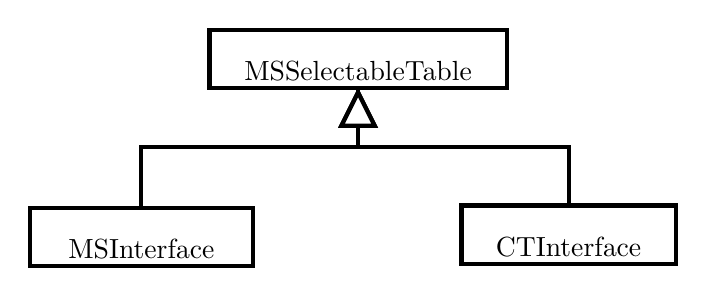
\begin{tikzpicture}
\pgftransformxscale{1.000000}
\pgftransformyscale{-1.000000}
\definecolor{dialinecolor}{rgb}{0.000000, 0.000000, 0.000000}
\pgfsetstrokecolor{dialinecolor}
\definecolor{dialinecolor}{rgb}{1.000000, 1.000000, 1.000000}
\pgfsetfillcolor{dialinecolor}
\pgfsetlinewidth{0.100000\du}
\pgfsetdash{}{0pt}
\definecolor{dialinecolor}{rgb}{1.000000, 1.000000, 1.000000}
\pgfsetfillcolor{dialinecolor}
\fill (16.450000\du,6.200000\du)--(16.450000\du,7.600000\du)--(23.607500\du,7.600000\du)--(23.607500\du,6.200000\du)--cycle;
\definecolor{dialinecolor}{rgb}{0.000000, 0.000000, 0.000000}
\pgfsetstrokecolor{dialinecolor}
\draw (16.450000\du,6.200000\du)--(16.450000\du,7.600000\du)--(23.607500\du,7.600000\du)--(23.607500\du,6.200000\du)--cycle;
% setfont left to latex
\definecolor{dialinecolor}{rgb}{0.000000, 0.000000, 0.000000}
\pgfsetstrokecolor{dialinecolor}
\node at (20.028750\du,7.200000\du){MSSelectableTable};
\pgfsetlinewidth{0.100000\du}
\pgfsetdash{}{0pt}
\definecolor{dialinecolor}{rgb}{1.000000, 1.000000, 1.000000}
\pgfsetfillcolor{dialinecolor}
\fill (12.120000\du,10.485000\du)--(12.120000\du,11.885000\du)--(17.497500\du,11.885000\du)--(17.497500\du,10.485000\du)--cycle;
\definecolor{dialinecolor}{rgb}{0.000000, 0.000000, 0.000000}
\pgfsetstrokecolor{dialinecolor}
\draw (12.120000\du,10.485000\du)--(12.120000\du,11.885000\du)--(17.497500\du,11.885000\du)--(17.497500\du,10.485000\du)--cycle;
% setfont left to latex
\definecolor{dialinecolor}{rgb}{0.000000, 0.000000, 0.000000}
\pgfsetstrokecolor{dialinecolor}
\node at (14.808750\du,11.485000\du){MSInterface};
\pgfsetlinewidth{0.100000\du}
\pgfsetdash{}{0pt}
\definecolor{dialinecolor}{rgb}{1.000000, 1.000000, 1.000000}
\pgfsetfillcolor{dialinecolor}
\fill (22.520000\du,10.435000\du)--(22.520000\du,11.835000\du)--(27.680000\du,11.835000\du)--(27.680000\du,10.435000\du)--cycle;
\definecolor{dialinecolor}{rgb}{0.000000, 0.000000, 0.000000}
\pgfsetstrokecolor{dialinecolor}
\draw (22.520000\du,10.435000\du)--(22.520000\du,11.835000\du)--(27.680000\du,11.835000\du)--(27.680000\du,10.435000\du)--cycle;
% setfont left to latex
\definecolor{dialinecolor}{rgb}{0.000000, 0.000000, 0.000000}
\pgfsetstrokecolor{dialinecolor}
\node at (25.100000\du,11.435000\du){CTInterface};
\pgfsetlinewidth{0.100000\du}
\pgfsetdash{}{0pt}
\pgfsetmiterjoin
\pgfsetbuttcap
{
\definecolor{dialinecolor}{rgb}{0.000000, 0.000000, 0.000000}
\pgfsetfillcolor{dialinecolor}
% was here!!!
\definecolor{dialinecolor}{rgb}{0.000000, 0.000000, 0.000000}
\pgfsetstrokecolor{dialinecolor}
\draw (20.028800\du,7.600000\du)--(20.028800\du,9.017320\du)--(14.808700\du,9.017320\du)--(14.808700\du,10.434600\du);
}
\definecolor{dialinecolor}{rgb}{0.000000, 0.000000, 0.000000}
\pgfsetstrokecolor{dialinecolor}
\draw (20.028800\du,8.511803\du)--(20.028800\du,9.017320\du)--(14.808700\du,9.017320\du)--(14.808700\du,10.434600\du);
\pgfsetmiterjoin
\definecolor{dialinecolor}{rgb}{1.000000, 1.000000, 1.000000}
\pgfsetfillcolor{dialinecolor}
\fill (20.428800\du,8.511803\du)--(20.028800\du,7.711803\du)--(19.628800\du,8.511803\du)--cycle;
\pgfsetlinewidth{0.100000\du}
\pgfsetdash{}{0pt}
\pgfsetmiterjoin
\definecolor{dialinecolor}{rgb}{0.000000, 0.000000, 0.000000}
\pgfsetstrokecolor{dialinecolor}
\draw (20.428800\du,8.511803\du)--(20.028800\du,7.711803\du)--(19.628800\du,8.511803\du)--cycle;
% setfont left to latex
\pgfsetlinewidth{0.100000\du}
\pgfsetdash{}{0pt}
\pgfsetmiterjoin
\pgfsetbuttcap
{
\definecolor{dialinecolor}{rgb}{0.000000, 0.000000, 0.000000}
\pgfsetfillcolor{dialinecolor}
% was here!!!
\definecolor{dialinecolor}{rgb}{0.000000, 0.000000, 0.000000}
\pgfsetstrokecolor{dialinecolor}
\draw (20.028800\du,7.600000\du)--(20.028800\du,9.017500\du)--(25.100000\du,9.017500\du)--(25.100000\du,10.435000\du);
}
\definecolor{dialinecolor}{rgb}{0.000000, 0.000000, 0.000000}
\pgfsetstrokecolor{dialinecolor}
\draw (20.028800\du,8.511803\du)--(20.028800\du,9.017500\du)--(25.100000\du,9.017500\du)--(25.100000\du,10.435000\du);
\pgfsetmiterjoin
\definecolor{dialinecolor}{rgb}{1.000000, 1.000000, 1.000000}
\pgfsetfillcolor{dialinecolor}
\fill (20.428800\du,8.511803\du)--(20.028800\du,7.711803\du)--(19.628800\du,8.511803\du)--cycle;
\pgfsetlinewidth{0.100000\du}
\pgfsetdash{}{0pt}
\pgfsetmiterjoin
\definecolor{dialinecolor}{rgb}{0.000000, 0.000000, 0.000000}
\pgfsetstrokecolor{dialinecolor}
\draw (20.428800\du,8.511803\du)--(20.028800\du,7.711803\du)--(19.628800\du,8.511803\du)--cycle;
% setfont left to latex
\end{tikzpicture}
